\chapter{NMR Proton}\label{ch:g12:proton-nmr}

Di sebuah rumah sakit, seorang pasien berbaring di dalam cincin pemindai
MRI, dan gambar jaringan lunak tubuhnya muncul di layar, yang disusun
dari jawaban inti-inti hidrogen dalam air dan lemak tubuhnya. Di sebuah
laboratorium kimia, sebuah tabung kaca kecil berisi beberapa miligram
senyawa diturunkan ke dalam lubang sebuah magnet yang kuat, dan sebuah
spektrum muncul, yang disusun dengan cara yang sama: magnet yang kuat,
sinyal radio, dan inti-inti hidrogen yang menjawabnya. Di dalam
spektrometer ahli kimia, setiap inti hidrogen menjawab sedikit berbeda
menurut tetangga-tetangganya, dan spektrumnya menjadi peta \omterm{def:g7:atoms-and-molecules:atom}{atom-atom}
hidrogen \omterm{def:g7:atoms-and-molecules:molecule}{molekul} itu.

\begin{recall}
\omterm{def:g11:infrared:spectrum}{Spektrum inframerah} memperlihatkan ikatan apa saja yang dimiliki sebuah
\omterm{def:g7:atoms-and-molecules:molecule}{molekul} (\cref{ch:g11:infrared}). \omterm{def:g11:functional-groups:functional-group}{Gugus fungsi}, keluarga senyawa, dan
\omterm{def:g11:organic-skeletons:isomer}{isomer} (\cref{ch:g11:functional-groups}, \cref{ch:g11:organic-skeletons}).
\end{recall}

\begin{omfigure}
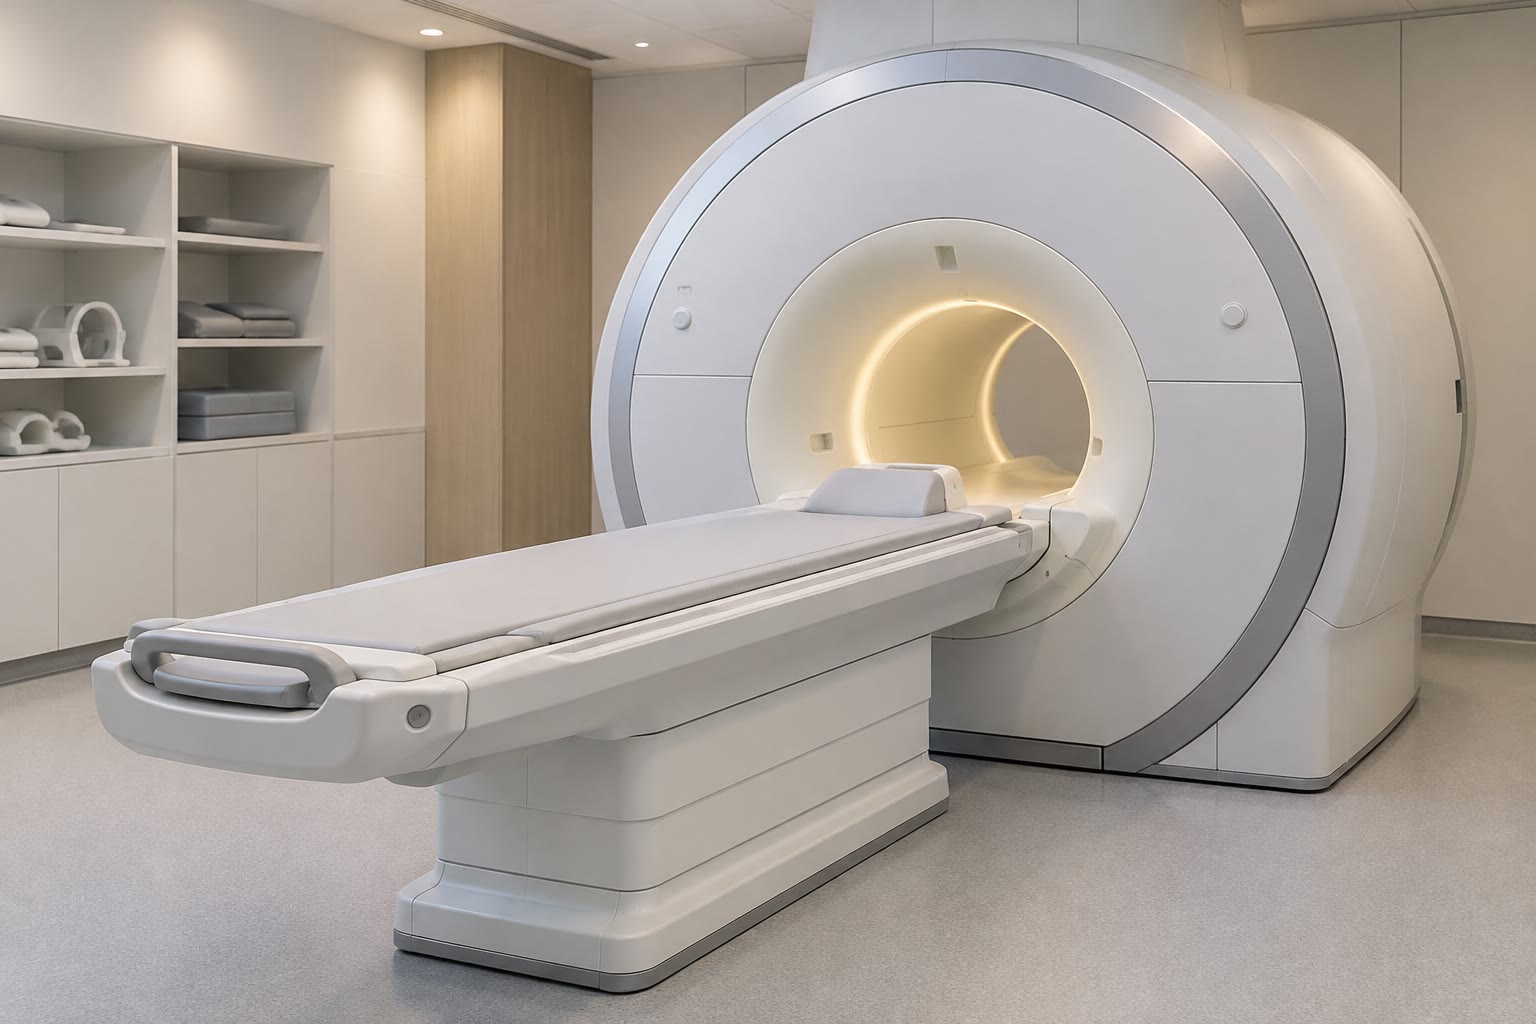
\includegraphics[width=0.48\linewidth]{images/book1/ai/g12-mri-room.jpg}

{\small Pemindai MRI: fisikanya sama dengan fisika spektrometer NMR
seorang ahli kimia.}
\end{omfigure}

\section{Proton dalam medan magnet}

\omterm{def:g9:inside-the-atom:nucleus}{Inti atom} hidrogen adalah sebuah \omterm{def:g9:inside-the-atom:proton}{proton} tunggal. Jika ditempatkan dalam
medan magnet yang kuat, \omterm{def:g9:inside-the-atom:proton}{proton} itu menyerap gelombang radio dengan
frekuensi tertentu; bagaimana dan mengapa hal itu terjadi termasuk ranah
fisika, dan tidak diperlukan di sini. Yang penting bagi ahli kimia ialah
bahwa \omterm{def:g9:inside-the-atom:nucleus}{elektron-elektron} di sekitar sebuah \omterm{def:g9:inside-the-atom:proton}{proton} sedikit melindunginya
dari medan itu, dan bahwa perlindungan ini bergantung pada \omterm{def:g7:atoms-and-molecules:atom}{atom-atom} di
dekatnya: \omterm{def:g9:inside-the-atom:proton}{proton} yang bersebelahan dengan \omterm{def:g7:atoms-and-molecules:atom}{atom} oksigen yang
elektronegatif, yang menarik \omterm{def:g9:inside-the-atom:nucleus}{elektron} menjauh, menyerap pada frekuensi
yang sedikit berbeda dari \omterm{def:g9:inside-the-atom:proton}{proton} dalam rantai hidrokarbon. Perbedaannya
sangat kecil, beberapa sepersejuta frekuensinya, dan dinyatakan dalam
bagian per juta.

\begin{omfigure}
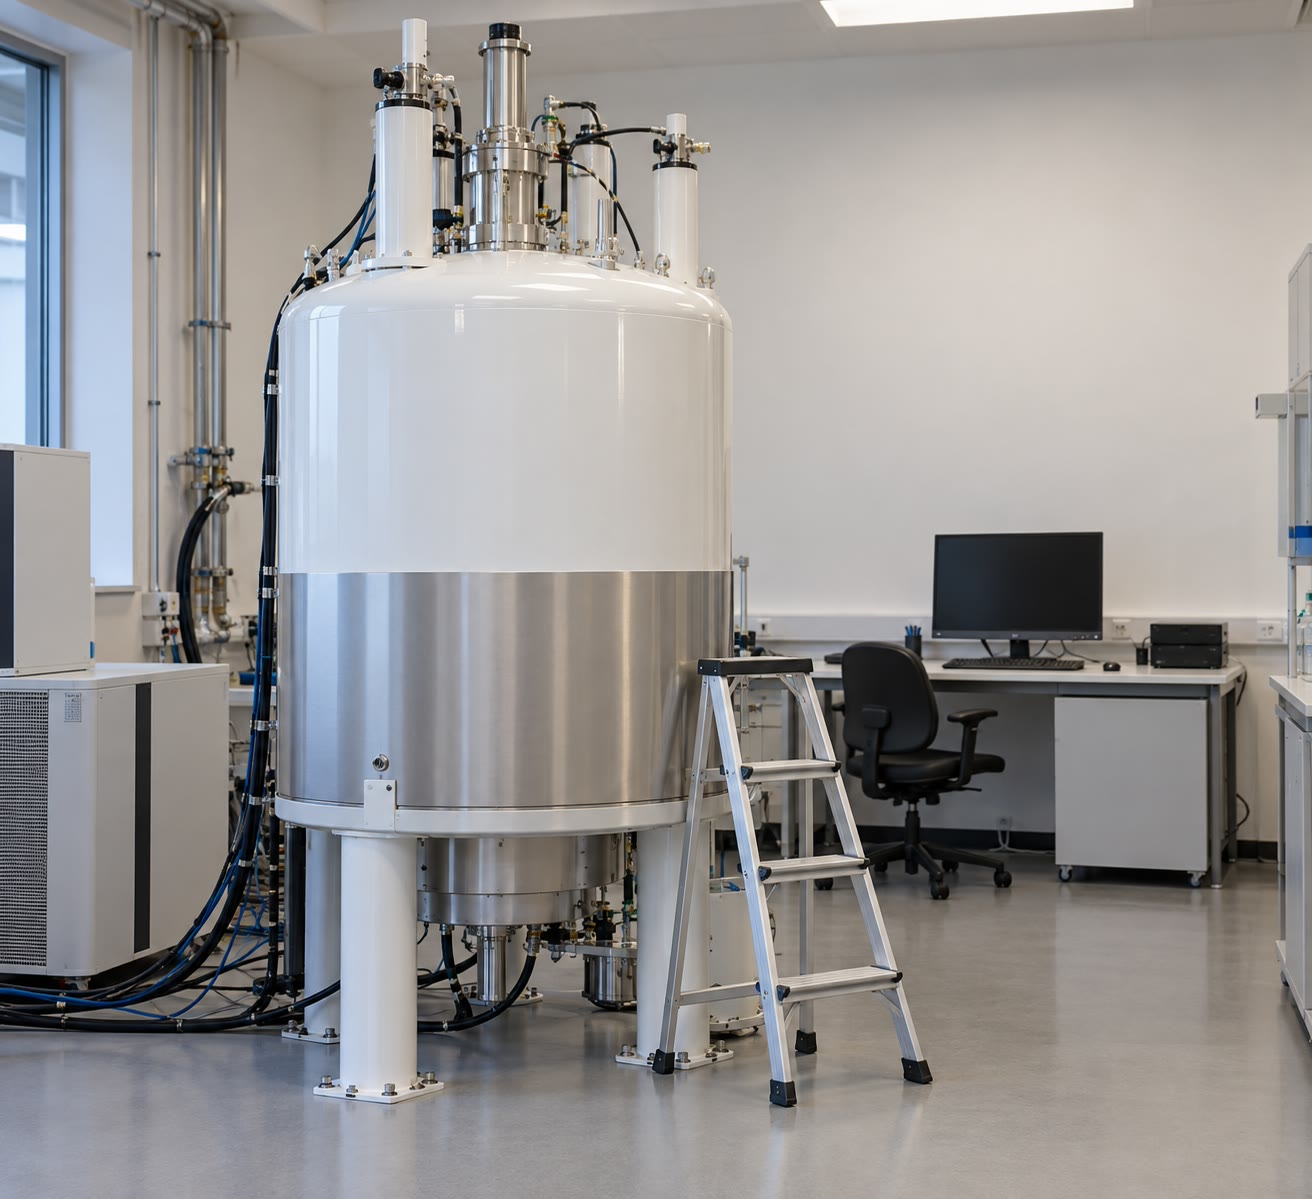
\includegraphics[width=0.42\linewidth]{images/book1/ai/g12-nmr-magnet.jpg}

{\small Magnet sebuah spektrometer NMR.}
\end{omfigure}

\begin{definition}[Spektrum NMR, pergeseran kimia]\label{def:g12:proton-nmr:spectrum}
Sebuah \emph{spektrum NMR}\index{spektrum NMR} \omterm{def:g9:inside-the-atom:proton}{proton} (resonansi
magnetik inti) memperlihatkan sinyal-sinyal yang diserap inti-inti
hidrogen sebuah senyawa. Posisi sebuah sinyal disebut
\emph{pergeseran kimia}\index{pergeseran kimia} $\delta$-nya, dalam
bagian per juta (\si{ppm}), yang diukur dari sinyal sebuah senyawa
acuan, tetrametilsilana \ce{Si(CH3)4} (TMS), yang ditetapkan pada
$\delta = 0$. Sumbu $\delta$ digambar membesar dari kanan ke kiri.
\end{definition}

\begin{proposition}[Pergeseran bergantung pada tetangga]\label{prop:g12:proton-nmr:shift}
% ledger: nmrr:CH3, nmrr:CH2, nmrr:allylic, nmrr:ketone, nmrr:halide, nmrr:alcohol, nmrr:vinylic, nmrr:aryl, nmrr:aldehyde, nmrr:acid
\omterm{def:g12:proton-nmr:spectrum}{Pergeseran kimia} sebuah \omterm{def:g9:inside-the-atom:proton}{proton} bergantung pada \omterm{def:g7:atoms-and-molecules:atom}{atom-atom} di dekatnya:
makin dekat \omterm{def:g9:inside-the-atom:proton}{proton} itu ke \omterm{def:g7:atoms-and-molecules:atom}{atom} yang elektronegatif atau ke \omterm{def:g10:lewis-and-shape:multiple-bond}{ikatan
rangkap}, makin besar pergeserannya. Rentang khasnya, dalam \si{ppm}:
\begin{center}
\small
\begin{tabular}{ll@{\qquad}ll}
\hline
lingkungan & $\delta$ & lingkungan & $\delta$ \\
\hline
\ce{CH3} dalam rantai & 0.7--1.3 & \ce{H-C-O} (\omterm{def:g11:functional-groups:alcohol}{alkohol}, eter, \omterm{def:g11:functional-groups:carboxylic-acid}{ester}) & 3.3--4.5 \\
\ce{CH2} dalam rantai & 1.2--1.6 & \ce{H-C=C} & 4.5--6.5 \\
\ce{H-C-C=C} & 1.6--2.2 & H pada cincin benzena & 6.5--8.0 \\
\ce{H-C-C=O} & 2.0--2.4 & \omterm{def:g11:functional-groups:carbonyl}{aldehida} \ce{-CHO} & 9.7--10.0 \\
\ce{H-C-X} (\omterm{def:g10:electron-shells:family}{halogen}) & 2.5--4.0 & asam \ce{-COOH} & 11.0--12.0 \\
\hline
\end{tabular}
\end{center}
\end{proposition}

\begin{proof}
Diukur pada banyak senyawa. Tetangga yang elektronegatif menarik
\omterm{def:g9:inside-the-atom:nucleus}{elektron} menjauh dari \omterm{def:g9:inside-the-atom:proton}{proton}, sehingga \omterm{def:g9:inside-the-atom:proton}{proton} itu kurang terlindungi dan
menyerap pada pergeseran yang lebih besar.
\end{proof}

\begin{omfigure}
\begin{tikzpicture}[font=\small, x=0.75cm, y=0.5cm]
  % delta axis reversed: x = 12 - delta
  \draw[->] (0,0) -- (12.4,0) node[right] {};
  \foreach \d in {12,11,10,9,8,7,6,5,4,3,2,1,0}
    \draw ({12-\d},0) -- ({12-\d},-0.2) node[below, font=\footnotesize] {\d};
  \node[below=14pt] at (6,-0.3) {$\delta$ (\si{ppm})};
  \foreach \a/\b/\y/\c/\l in {
      11.0/12.0/1/omThm/{\ce{COOH}},
      9.7/10.0/2/omThm/{\ce{CHO}},
      6.5/8.0/1/black!60/{cincin benzena},
      4.5/6.5/2/omMeth/{\ce{C=C-H}},
      3.3/4.5/3/omDef/{\ce{H-C-O}},
      2.0/2.4/4/omProp/{\ce{H-C-C=O}},
      0.7/1.6/5/black!45/{\ce{CH3}, \ce{CH2} rantai}} {
    \fill[\c, rounded corners=1pt] ({12-\b},{\y-0.3}) rectangle ({12-\a},{\y+0.3});
    \node[anchor=west, font=\footnotesize] at ({12-\a+0.1},\y) {\l};
  }
  \draw[thick] (12,0) -- (12,0.6) node[above, font=\footnotesize] {TMS};
\end{tikzpicture}

{\small Tempat \omterm{def:g9:inside-the-atom:proton}{proton} menyerap, menurut lingkungannya. \omterm{def:g9:inside-the-atom:proton}{Proton} yang dekat
dengan oksigen, dengan \omterm{def:g10:lewis-and-shape:multiple-bond}{ikatan rangkap}, atau dengan gugus asam muncul di
sebelah kiri spektrum.}
\end{omfigure}

\begin{inthelab}[Menyiapkan tabung NMR]
Beberapa miligram senyawa dilarutkan dalam sekitar \qty{0.6}{mL}
\omterm{def:g6:solutions-and-solubility:solute}{pelarut} yang \omterm{def:g7:atoms-and-molecules:atom}{atom-atom} hidrogennya telah diganti dengan deuterium
(\ce{CDCl3}, kloroform terdeuterasi), yang tidak memberikan sinyal;
sedikit TMS ditambahkan sebagai acuan. Larutannya disaring ke dalam
tabung kaca tipis, yang kemudian ditutup, diberi label, dan diturunkan
ke dalam magnet.
\end{inthelab}

\section{Proton ekuivalen}

\begin{definition}[Proton ekuivalen]\label{def:g12:proton-nmr:equivalent}
\omterm{def:g9:inside-the-atom:proton}{Proton-proton} disebut \emph{proton ekuivalen}\index{proton ekuivalen}
jika memiliki lingkungan yang sama dalam \omterm{def:g7:atoms-and-molecules:molecule}{molekul}, sehingga menyerap pada
pergeseran yang sama. Setiap kelompok \omterm{def:g9:inside-the-atom:proton}{proton} ekuivalen memberikan satu
sinyal. Ketiga \omterm{def:g9:inside-the-atom:proton}{proton} sebuah gugus \ce{CH3} selalu ekuivalen.
\end{definition}

\begin{example}[Menghitung kelompok]\label{ex:g12:proton-nmr:groups}
Propanon, \ce{CH3-CO-CH3}, memiliki enam \omterm{def:g9:inside-the-atom:proton}{proton} tetapi hanya satu
kelompok: kedua gugus \ce{CH3}-nya serupa, masing-masing di satu sisi
gugus \ce{C=O}. Etanol, \ce{CH3-CH2-OH}, memiliki tiga kelompok (\ce{CH3},
\ce{CH2}, \ce{OH}). Etil etanoat, \ce{CH3-CO-O-CH2-CH3}, juga memiliki
tiga:
\ce{CH3} di sebelah \ce{C=O}, \ce{CH2} di sebelah \ce{O}, dan \ce{CH3}
di ujung.
\end{example}

\section{Integrasi}

\begin{definition}[Kurva integrasi]\label{def:g12:proton-nmr:integration}
Yang disebut \emph{kurva integrasi}\index{kurva integrasi} sebuah
\omterm{def:g12:proton-nmr:spectrum}{spektrum NMR} adalah kurva, yang digambar di atas sinyal-sinyal, yang
naik satu anak tangga pada setiap sinyal: tinggi setiap anak tangga
sebanding dengan jumlah \omterm{def:g9:inside-the-atom:proton}{proton} yang memberikan sinyal itu.
\end{definition}

\begin{example}[Membaca anak tangga]\label{ex:g12:proton-nmr:steps}
Dalam spektrum etanol, anak tangga di atas ketiga sinyal berukuran 2, 1,
dan 3 satuan, dari kiri ke kanan: \ce{CH2}, \ce{OH}, dan \ce{CH3}. Hanya
perbandingannya yang penting: anak tangga 12, 6, dan 18 mm menyatakan
hal yang sama.
\end{example}

\section{Multiplisitas dan aturan \texorpdfstring{$n+1$}{n+1}}


\begin{definition}[Multiplet, aturan $n+1$]\label{def:g12:proton-nmr:multiplet}
Sebuah sinyal sering terpecah menjadi beberapa garis yang berdekatan:
sebuah \emph{multiplet}\index{multiplet} (singlet, doblet, triplet,
kuartet, \dots{} untuk 1, 2, 3, 4 garis). Menurut
\emph{aturan $n+1$}\index{aturan n+1@aturan $n+1$}, sekelompok \omterm{def:g12:proton-nmr:equivalent}{proton
ekuivalen} yang \omterm{def:g7:atoms-and-molecules:atom}{atom-atom} karbon tetangganya membawa seluruhnya $n$
\omterm{def:g9:inside-the-atom:proton}{proton}, yang tidak ekuivalen dengannya, memberikan sinyal dengan $n+1$
garis, dengan intensitas yang perbandingannya mengikuti segitiga Pascal.
\end{definition}

\begin{proposition}[Pemecahan oleh tetangga]\label{prop:g12:proton-nmr:n-plus-one}
Dalam \omterm{def:g7:atoms-and-molecules:molecule}{molekul} \ce{CH3-CH2-X} (X tanpa hidrogen), sinyal \ce{CH3} berupa
triplet (2 \omterm{def:g9:inside-the-atom:proton}{proton} tetangga) dan sinyal \ce{CH2} berupa kuartet (3 \omterm{def:g9:inside-the-atom:proton}{proton}
tetangga). \omterm{def:g9:inside-the-atom:proton}{Proton} yang terikat pada \omterm{def:g7:atoms-and-molecules:atom}{atom} oksigen atau nitrogen biasanya
memberikan singlet dan tidak memecah sinyal tetangganya.
\end{proposition}

\begin{proof}
Diterima tanpa bukti: setiap \omterm{def:g9:inside-the-atom:proton}{proton} tetangga sedikit menggeser sinyal ke
atas atau ke bawah menurut keadaannya sendiri, dan kombinasinya
memberikan $n+1$ garis; fisikanya dijelaskan dalam buku Tahun Pertama
universitas. \omterm{def:g9:inside-the-atom:proton}{Proton} pada O atau N dipertukarkan dengan cepat antarmolekul,
sehingga pengaruhnya terhapus secara rata-rata.
\end{proof}

\begin{omfigure}
\begin{tikzpicture}[font=\small]
  % Pascal's triangle
  \foreach \r/\vals in {0/{1}, 1/{1,1}, 2/{1,2,1}, 3/{1,3,3,1}, 4/{1,4,6,4,1}} {
    \foreach \v [count=\i from 0] in \vals
      \node at ({\i*0.7 - \r*0.35}, {-\r*0.55}) {\v};
    \node[anchor=east, font=\footnotesize, black!60] at (-2.0,{-\r*0.55}) {$n = \r$};
  }
  % multiplets
  \begin{scope}[xshift=4.2cm, yshift=-2.4cm]
    \foreach \x/\name/\hs in {0/singlet/{1}, 1.4/doblet/{1,1}, 3.0/triplet/{1,2,1},
                              4.9/kuartet/{1,3,3,1}} {
      \foreach \h [count=\i from 0] in \hs {
        \draw[very thick, omDef] ({\x + \i*0.22},0) -- ({\x + \i*0.22},{\h*0.55});
      }
      \node[anchor=north, font=\footnotesize] at ({\x+0.3},-0.1) {\name};
    }
  \end{scope}
\end{tikzpicture}

{\small Segitiga Pascal memberikan intensitas relatif $n+1$ garis sebuah
sinyal yang dipecah oleh $n$ \omterm{def:g9:inside-the-atom:proton}{proton} tetangga: 1:1, 1:2:1, 1:3:3:1.}
\end{omfigure}

\begin{omfigure}
\newcommand{\nmrpanel}[4]{% file part, title, xmax, ymax
\begin{tikzpicture}
\begin{axis}[width=\linewidth, height=4.2cm, x dir=reverse, xmin=0,
    xmax=#3, ymin=0, ymax=#4, ytick=\empty, axis y line=none,
    axis x line*=bottom, xlabel={$\delta$ (\si{ppm})},
    tick label style={font=\scriptsize}, label style={font=\scriptsize},
    title={\small #2}, title style={yshift=-3pt}]
  \addplot[omDef, thin] table[x=delta, y=I] {figdata/out/grade-12-proton-nmr-#1.dat};
  \addplot[omProp, thick] table[x=delta, y expr=0.15+\thisrow{integral}*0.11]
    {figdata/out/grade-12-proton-nmr-#1.dat};
\end{axis}
\end{tikzpicture}}
\begin{minipage}{0.49\linewidth}\nmrpanel{a}{A: etanol}{5}{1.15}\end{minipage}\hfill
\begin{minipage}{0.49\linewidth}\nmrpanel{b}{B: etil etanoat}{5}{1.15}\end{minipage}

\begin{minipage}{0.49\linewidth}\nmrpanel{c}{C: propanon}{5}{1.15}\end{minipage}\hfill
\begin{minipage}{0.49\linewidth}\nmrpanel{e}{D: metil etanoat}{5}{1.15}\end{minipage}

\begin{minipage}{\linewidth}\nmrpanel{d}{E: asam propanoat}{12.5}{1.15}\end{minipage}

{\small \omterm{def:g12:proton-nmr:spectrum}{Spektrum NMR} \omterm{def:g9:inside-the-atom:proton}{proton} (biru) dengan \omterm{def:g12:proton-nmr:integration}{kurva integrasinya} (jingga;
setiap anak tangga sebanding dengan jumlah \omterm{def:g9:inside-the-atom:proton}{proton} sinyal di bawahnya).
Pergeserannya adalah pergeseran spektrum terukur dalam \ce{CDCl3};
bentuk dan jarak garisnya digambar dari sebuah model sederhana.}
\end{omfigure}

\begin{example}[Membaca spektrum]\label{ex:g12:proton-nmr:reading}
% ledger: nmr:ethylethanoate-OCH2, nmr:ethylethanoate-COCH3, nmr:ethylethanoate-CH3, nmr:ethanol-CH2, nmr:ethanol-CH3, nmr:ethanol-OH, nmr:acetone, nmr:propanoic-CH2, nmr:propanoic-CH3, nmr:propanoic-OH, nmr:meoac-OCH3, nmr:meoac-COCH3
Etil etanoat (B) memberikan kuartet 2 \omterm{def:g9:inside-the-atom:proton}{proton} pada \qty{4.12}{ppm}
(\ce{O-CH2}, di sebelah oksigen dan sebuah \ce{CH3}), singlet 3 \omterm{def:g9:inside-the-atom:proton}{proton}
pada \qty{2.04}{ppm} (\ce{CH3-C=O}, tanpa \omterm{def:g9:inside-the-atom:proton}{proton} tetangga), dan triplet
3 \omterm{def:g9:inside-the-atom:proton}{proton} pada \qty{1.26}{ppm} (\ce{CH3}, di sebelah sebuah \ce{CH2}).
Propanon (C) hanya memberikan satu singlet 6 \omterm{def:g9:inside-the-atom:proton}{proton} pada
\qty{2.16}{ppm}. Asam propanoat (E) memiliki kuartet pada
\qty{2.39}{ppm}, triplet pada \qty{1.16}{ppm}, dan singlet jauh di
kiri, pada \qty{11.7}{ppm}, yaitu \omterm{def:g9:inside-the-atom:proton}{proton} asamnya.
\end{example}

\section{Memakai inframerah dan NMR bersama-sama}


\begin{method}[Mengenali molekul dari spektrum IR dan NMR-nya]\label{met:g12:proton-nmr:identify}
\begin{enumerate}
  \item Dari \omterm{def:g11:organic-skeletons:formulas}{rumus molekulnya}, daftarlah \omterm{def:g11:organic-skeletons:isomer}{isomer-isomer} yang mungkin
        beserta \omterm{def:g11:functional-groups:functional-group}{gugus fungsinya}.
  \item Inframerah: carilah pita \ce{C=O} di dekat \qty{1700}{cm^{-1}}
        serta pita \ce{O-H} atau \ce{N-H}; coretlah \omterm{def:g11:organic-skeletons:isomer}{isomer} yang tidak
        cocok.
  \item NMR: hitunglah sinyalnya (kelompok \omterm{def:g12:proton-nmr:equivalent}{proton ekuivalen}), bacalah
        integrasinya (jumlah \omterm{def:g9:inside-the-atom:proton}{proton} per kelompok), multiplisitasnya
        (tetangga), dan pergeserannya (lingkungan).
  \item Rangkailah potongan-potongan itu menjadi satu struktur, lalu
        periksalah struktur itu terhadap setiap pengamatan.
\end{enumerate}
\end{method}

\begin{example}[Dua isomer \ce{C3H6O2}]\label{ex:g12:proton-nmr:isomers}
Asam propanoat \ce{CH3-CH2-COOH} dan metil etanoat \ce{CH3-CO-O-CH3}
adalah \omterm{def:g11:organic-skeletons:isomer}{isomer}. Dalam inframerah, hanya asamnya yang memperlihatkan pita
\ce{O-H} yang sangat lebar. Dalam NMR (spektrum E dan D), asamnya
memberikan triplet, kuartet, dan singlet di dekat \qty{11.7}{ppm};
\omterm{def:g11:functional-groups:carboxylic-acid}{esternya} memberikan dua singlet yang masing-masing 3 \omterm{def:g9:inside-the-atom:proton}{proton}, pada 3.66
(\ce{O-CH3}) dan \qty{2.05}{ppm} (\ce{CH3-C=O}), karena tidak ada \omterm{def:g7:atoms-and-molecules:atom}{atom}
karbon \omterm{def:g11:functional-groups:carboxylic-acid}{ester} itu yang membawa \omterm{def:g9:inside-the-atom:proton}{proton} di sebelah karbon lain yang
berproton.
\end{example}

\section{Latihan}

\begin{exercise}[$\star$]\label{exo:g12:proton-nmr:1}
Berapa kelompok \omterm{def:g12:proton-nmr:equivalent}{proton ekuivalen}, dan jadi berapa sinyal, yang
diberikan \omterm{def:g7:atoms-and-molecules:molecule}{molekul-molekul} ini: metana; etana \ce{CH3-CH3}; propana;
metanol \ce{CH3-OH}; metoksimetana \ce{CH3-O-CH3}?
\end{exercise}

\begin{exercise}[$\star$]\label{exo:g12:proton-nmr:2}
Sekelompok \omterm{def:g9:inside-the-atom:proton}{proton} memiliki 2 \omterm{def:g9:inside-the-atom:proton}{proton} tetangga pada karbon sebelahnya.
Berapa garis sinyalnya, dan dengan perbandingan berapa? Pertanyaan yang
sama untuk 3 dan untuk 0 tetangga.
\end{exercise}

\begin{exercise}[$\star$]\label{exo:g12:proton-nmr:3}
Sebuah spektrum memiliki tiga sinyal dengan anak tangga integrasi 15,
10, dan 15 mm. \omterm{def:g7:atoms-and-molecules:molecule}{Molekulnya} memiliki 8 \omterm{def:g9:inside-the-atom:proton}{proton}. Berapa \omterm{def:g9:inside-the-atom:proton}{proton} yang
diwakili setiap sinyal?
\end{exercise}

\begin{exercise}[$\star$]\label{exo:g12:proton-nmr:4}
Dengan tabel pergeseran, di mana kamu perkirakan sinyal \omterm{def:g9:inside-the-atom:proton}{proton} gugus
\omterm{def:g11:functional-groups:carbonyl}{aldehida}? Sinyal gugus \ce{CH3} dalam rantai?
\end{exercise}

\begin{exercise}[$\star$]\label{exo:g12:proton-nmr:5}
Mengapa acuan TMS dipilih sehingga semua \omterm{def:g9:inside-the-atom:proton}{protonnya} ekuivalen? Mengapa
\omterm{def:g6:solutions-and-solubility:solute}{pelarutnya} terdeuterasi?
\end{exercise}

\begin{exercise}[$\star\star$]\label{exo:g12:proton-nmr:6}
Ramalkan spektrum kloroetana \ce{CH3-CH2-Cl}: jumlah sinyal, integrasi,
multiplisitas, pergeseran perkiraan.
\end{exercise}

\begin{exercise}[$\star\star$]\label{exo:g12:proton-nmr:7}
Ramalkan spektrum propan-2-ol, \ce{(CH3)2CH-OH}: khususnya,
multiplisitas sinyal \ce{CH3} dan sinyal \ce{CH} (anggaplah \ce{OH}
memberikan singlet dan tidak memecah sinyal lain).
\end{exercise}

\begin{exercise}[$\star\star$]\label{exo:g12:proton-nmr:8}
Tiga spektrum: (a) satu singlet; (b) kuartet, singlet, dan triplet,
integrasi 2:3:3; (c) kuartet, triplet, dan singlet jauh di kiri,
integrasi 2:3:1. Pasangkan spektrum-spektrum itu dengan etil etanoat,
propanon, dan asam propanoat.
\end{exercise}

\begin{exercise}[$\star\star$]\label{exo:g12:proton-nmr:9}
Dengan peta pergeseran, jelaskan mengapa \ce{CH2} etil etanoat
(\qty{4.12}{ppm}) jauh di sebelah kiri \ce{CH3} gugus etil yang sama
(\qty{1.26}{ppm}).
\end{exercise}

\begin{exercise}[$\star\star$]\label{exo:g12:proton-nmr:10}
Sebuah senyawa \ce{C3H6O} memperlihatkan pita inframerah yang kuat pada
\qty{1715}{cm^{-1}} dan satu singlet NMR saja. Kenalilah senyawa itu.
Mengapa propanal tidak mungkin?
\end{exercise}

\begin{exercise}[$\star\star$]\label{exo:g12:proton-nmr:11}
Dalam spektrum etanol, mengapa sinyal \ce{OH} berupa singlet, dan
mengapa \ce{CH2} muncul sebagai kuartet, bukan sebagai sinyal yang
lebih rumit?
\end{exercise}

\begin{exercise}[$\star\star\star$]\label{exo:g12:proton-nmr:12}
Berikan struktur empat \omterm{def:g11:organic-skeletons:isomer}{isomer} \ce{C4H8O2} yang berupa \omterm{def:g11:functional-groups:carboxylic-acid}{ester} atau asam
(asam butanoat, etil etanoat, metil propanoat, propil metanoat,
\dots), lalu ramalkan, untuk masing-masing, jumlah sinyal NMR dan
multiplisitasnya.
\end{exercise}

\begin{exercise}[$\star\star\star$]\label{exo:g12:proton-nmr:13}
Setetes air berat \ce{D2O} dikocok dengan larutan etanol, lalu
spektrumnya direkam lagi: satu sinyal menghilang. Sinyal yang mana, dan
mengapa? Bagaimana hal ini membantu mengenali \omterm{def:g9:inside-the-atom:proton}{proton} \ce{O-H}?
\end{exercise}

\begin{exercise}[$\star\star\star$]\label{exo:g12:proton-nmr:14}
Sebuah sampel etil etanoat mengandung sedikit etanol. Sinyal tambahan
apa yang muncul dalam spektrumnya? Jika integrasi singlet pada
\qty{2.04}{ppm} adalah 30 mm dan integrasi sebuah triplet tambahan kecil
pada \qty{1.23}{ppm} adalah 3 mm, perkirakan perbandingan jumlah etanol
dan \omterm{def:g11:functional-groups:carboxylic-acid}{ester}.
\end{exercise}

\begin{exercise}[$\star\star\star$]\label{exo:g12:proton-nmr:15}
2-Metilpropan-1-ol adalah \ce{(CH3)2CH-CH2-OH}. Ramalkan spektrumnya:
sinyal-sinyalnya, integrasinya, dan multiplisitas sinyal \ce{CH3} dan
\ce{CH2}. Sinyal mana yang memiliki garis paling banyak?
\end{exercise}

\section{Soal: Pelarut yang Tak Dikenal}

\begin{problem}[{Soal akhir pekan --- sebotol \omterm{def:g6:solutions-and-solubility:solute}{pelarut} yang hanya berlabel
\ce{C4H8O2}: zat apakah itu, dan berapa tinggi setiap anak tangga \omterm{def:g12:proton-nmr:integration}{kurva
integrasinya}?}]
\label{pb:g12:proton-nmr:1}
% ledger: nmr:ethylethanoate-OCH2, nmr:ethylethanoate-COCH3, nmr:ethylethanoate-CH3, ir:CO-ester, ir:OH-acid
Sebotol \omterm{def:g6:solutions-and-solubility:solute}{pelarut} di gudang hanya berlabel ``\ce{C4H8O2}''. \omterm{def:g11:infrared:spectrum}{Spektrum
inframerahnya} memperlihatkan pita yang kuat pada \qty{1740}{cm^{-1}} dan
tidak ada pita di atas \qty{3100}{cm^{-1}}. \omterm{def:g12:proton-nmr:spectrum}{Spektrum NMR-nya}
memperlihatkan tiga sinyal: kuartet pada \qty{4.12}{ppm}, singlet pada
\qty{2.04}{ppm}, dan triplet pada \qty{1.26}{ppm}. \omterm{def:g12:proton-nmr:integration}{Kurva integrasinya}
naik seluruhnya \qty{72}{mm}.

\medskip
\noindent\textbf{Bagian I --- Calon-calonnya.}
\begin{enumerate}
  \item Periksalah bahwa \ce{C4H8O2} cocok untuk sebuah \omterm{def:g11:functional-groups:carboxylic-acid}{ester} atau \omterm{def:g11:functional-groups:carboxylic-acid}{asam
        karboksilat} yang rantainya hanya berikatan tunggal.
  \item Berikan \omterm{def:g11:organic-skeletons:formulas}{rumus struktur ringkas} dan nama asam butanoat serta
        ketiga \omterm{def:g11:functional-groups:carboxylic-acid}{ester} etil etanoat, metil propanoat, dan propil
        metanoat.
  \item \omterm{def:g11:functional-groups:functional-group}{Gugus fungsi} apa yang dimiliki bersama oleh pasangan-pasangannya?
\end{enumerate}

\medskip
\noindent\textbf{Bagian II --- Inframerah.}
\begin{enumerate}[resume]
  \item Apa yang diungkapkan pita pada \qty{1740}{cm^{-1}}?
  \item Apa yang akan diperlihatkan asam butanoat tetapi tidak ada di
        sini? Coretlah asam itu.
  \item Dapatkah inframerah saja memilih di antara ketiga \omterm{def:g11:functional-groups:carboxylic-acid}{ester} itu?
\end{enumerate}

\medskip
\noindent\textbf{Bagian III --- NMR.}
\begin{enumerate}[resume]
  \item Berapa kelompok \omterm{def:g12:proton-nmr:equivalent}{proton ekuivalen} yang dimiliki senyawa yang tak
        dikenal itu?
  \item Apa yang ditunjukkan kuartet dan triplet itu bersama-sama?
  \item Apa yang dikatakan singlet itu tentang tetangga \omterm{def:g9:inside-the-atom:proton}{proton-protonnya}?
  \item Mengapa kuartet itu berada pada pergeseran yang besar?
  \item Ramalkan spektrum metil propanoat \ce{CH3-CH2-CO-O-CH3}
        (sinyal, multiplisitas, pergeseran perkiraan). Apakah itu senyawa
        yang dicari?
  \item Ramalkan spektrum propil metanoat. Apakah itu senyawa yang
        dicari?
\end{enumerate}

\medskip
\noindent\textbf{Bagian IV --- Identifikasi dan integrasi.}
\begin{enumerate}[resume]
  \item Kenalilah senyawa yang tak dikenal itu dan gambarlah
        strukturnya, dengan memberi label pada setiap sinyal.
  \item Berapa \omterm{def:g9:inside-the-atom:proton}{proton} yang diwakili setiap sinyal?
  \item Integrasi totalnya \qty{72}{mm} untuk 8 \omterm{def:g9:inside-the-atom:proton}{proton}. Berapa milimeter
        per \omterm{def:g9:inside-the-atom:proton}{proton}?
  \item Hitung tinggi anak tangga singlet dan triplet.
  \item Periksalah bahwa jumlah ketiga anak tangga itu \qty{72}{mm}.
  \item Etil etanoat berbau seperti permen buah pir: apakah hal itu
        sesuai dengan keluarga senyawa yang ditemukan?
  \item Nyatakan jawaban akhirnya: berapa tinggi anak tangga integrasi
        kuartet itu?
\end{enumerate}
\end{problem}
